
\status{Mostly written}

As explained in chapter \ref{chap:background},
Mercury manages its parallel work with userspace scheduling.
Engines execute context and switching contexts is done in userspace.
Each Mercury engine corresponds to an operating system thread such as a
POSIX thread\cite{butenhof1997:pthreads}.
The operating system manages these threads including their mapping onto
processors.

\plan{Introduce SMT}

\plan{Explain why we want $P$ engines when there are $P$ processors}
In order to make use of each of the system's processors we should create at
least one thread for each processor.
Creating more than one thread per processor consumes more resources
than necessary,
and when more than one thread is actively using the same processor the
operating system must perform context switches between these threads.
Therefore it is best to use exactly one thread per processor,
which is the default.
\plan{Explain briefly how we detect how many processors there are,}
We have been using the \code{sysconf} system call to detect the number of
processors in the system.
This is supported on several but not all platforms.
If Mercury cannot detect the number of processors in the system it defaults 
to useing a single engine.

\plan{Explain why we want thread pinning.}
We have been relying on the operating system to assign threads onto
processors.
This is usually acceptable,
but it is generally considered more reliable to pin threads to specific
processors.
%This is beginning to become more important as processors are made with
%larger numbers of cores and therefore more complex memory hierarchies.
\plan{Explain how we get thread pinning.}
We can \emph{pin} a thread to a specific processor using the
\code{setcpuaffiny()} system call,
which is available on many Unix-like OSs.
Our initial thread pinning implementation pinned each of Mercury's engines
to a separate processor.
The goals are to ensure that two thread are not contending for the same
processor, leaving another processor idle;
and that threads are not needlessly migrated between processors.
Thread pinning should also work when the user requests fewer engines
than processors.
When the user requests more engines than processors,
only the first $P$ thread are pinned (where there are $P$ processors).

\paul{Initial results here}

\plan{Benchmarks}

\plan{Problem with SMT}

\begin{figure}
\begin{center}
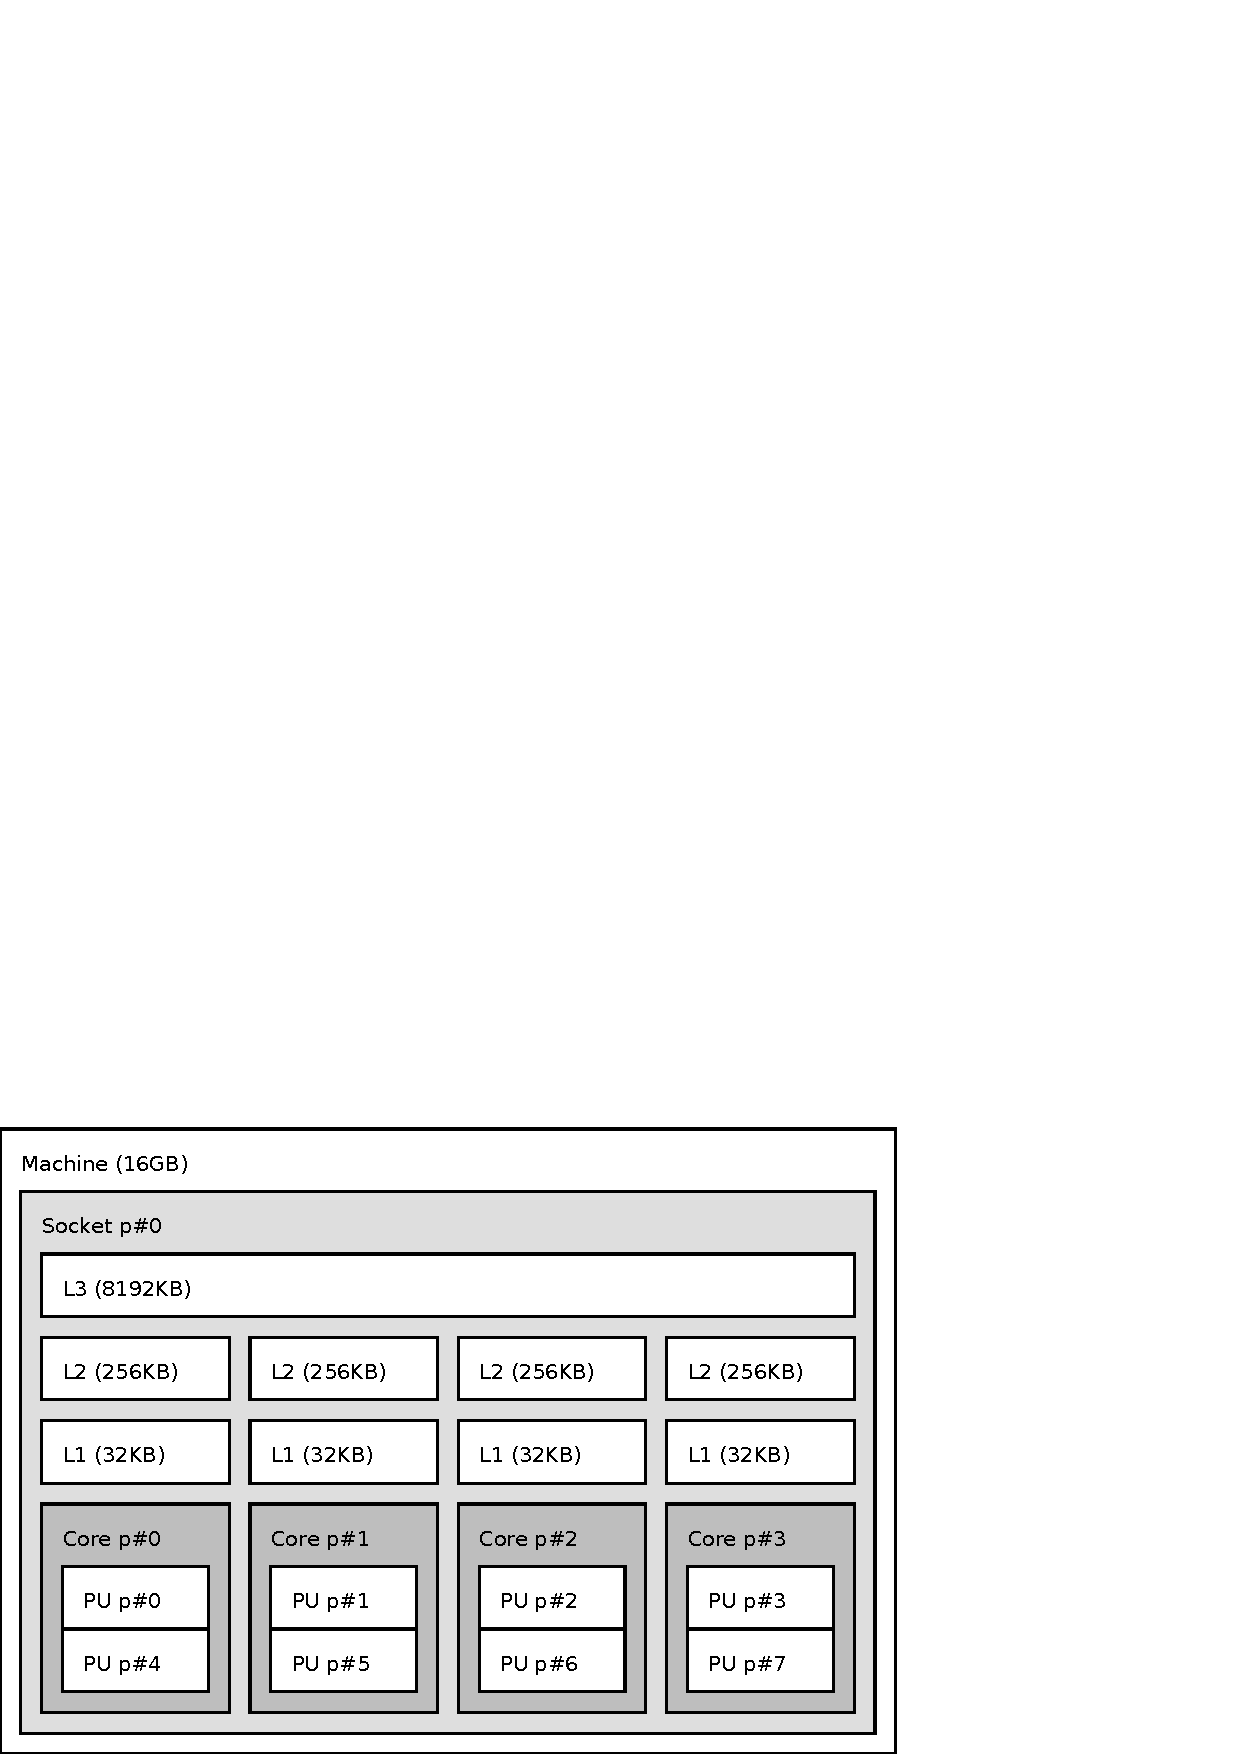
\includegraphics[width=0.75\textwidth]{i7-hierarchy}
\end{center}
\caption{Memory hierarchy of the Intel i7-2600K processor and 16GB of main
memory}
\label{fig:i7_hierarchy}
\end{figure}

\plan{What about SMT, not all processors are equal.}
This works well on SMP systems that do not use SMT.
On systems that use SMP and SMT
\footnote{
    SMT is sometimes called ``hyperthreading'' especially for marketing.}
(symmetric multithreading) as well as SMP this causes problems.
Consider the memory hierarchy of the Intel i7-2600K processor
(figure \ref{fig:i7_hierarchy}).
The i7-2600K has four cores, each with two hardware threads,
program units (PUs) in the figure.
If Mercury successfully detects that the system has eight logical processors
or the user specifies eight engines then thread pinning will correctly pin
each engine to a separate thread.
However,
if the user requests only four engines, which cores will be used?
depending on how they are selected,
and how the OS's \code{setcpuaffinity()} system call labels them,
all four Mercury engines could be pinned to just two of the CPU's cores
instead of being distributed uniformly across all four cores.
Uniform distribution will result in higher performance for the Mercury
program,
but it may affect other processes running on the same system.

\plan{How do we handle SMT}
Unfortunately there is no method provided by all operating systems to
determine the system's memory hierarchy.
Therefore we use a third party library
named Portable Hardware Locality (hwloc) \citep{broquedis:2010:hwloc}.
Hwloc provides some tools such as the one that drew figure
\ref{fig:i7_hierarchy},
but more importantly it provides an API for querying the memory hierarchy of
the system and methods for pinning threads to (sets of) cores or hardware
threads.
We use hwloc to determine the number of hardware threads in a system,
and optionally pin engines to hardware threads.
If the user specified the number of engines to use,
then we pin each engine to a hardware thread in each core so that engines
are distributed to cores as evenly as possible.
If the user specifies more engines than are available
(which we admit would be silly) then we allow more than one engine per
hardware thread,
meanwhile keeping engines as evenly distributed as possible amongst the
threads and cores.


%\plan{Further work}
%As we discussed in the previous section,
%knowledge of the memory hierarchy could help make better scheduling
%decisions.
%When using thread pinning we can guarantee that a particular engine is
%running on a particular processor/hardware thread,
%combining this with information about the memory hierarchy such as shared
%caches/sockets we can know which processors share the same cache(s) with the
%current processor either prefer to steal work from them or send work to
%them.

